\begin{savequote}[10cm] % this sets the width of the quote
\sffamily
Quote

\qauthor{quote author}
\end{savequote}

\chapter{Experiment}





\section{Research Objective}
This survey was devised to ascertain the quality of internet access across a range of locations and the effect of the internet on the dimensions of experience that are relevant to this thesis, namely Health and Well-being, Culture and Society and participation in the Economy. 
\section{Hypothesis}
My assumption was that access to the internet and the quality of that access made and makes a material difference to the quality of life of those people who can access it in the five dimensions of cultural and social interaction and participation, health and emotional well-being and economic well-being.
\section{Methods}
The survey was conducted by commissioning an organisation, \index{Qualtrics} Qualtrics, to administer the survey with certain parameters. This organisation was selected as it was one that is already used by Macquarie University for survey tools for social science surveys and because they have recently started recruiting general purpose Australian survey panels having opened an office in Australia. Qualtrics paid participants for completing their surveys according to their agreement with them. Funding was limited to \$5,000 which was obtained through a research grant made available by the Department of Computer Science at Macquarie University. The survey was administered in five regions denoted by Australian Bureau of Statistics (ABS) remoteness categories: Major Cities of Australia (MCA), Inner Regional Areas (IRA), Outer Regional Areas (ORA), Remote Areas of Australia (RA) and Very Remote Areas of Australia (VRA). I decided to use these areas to correlate results from this survey with similar results from the ABS in the same regional areas. These areas were determined by the respondent identifying their postcode which the ABS had already classified according to these remoteness characteristics. In some cases the respondent may have a different postcode to the GPS coordinates of the internet location at which they lodged the survey. This may be due to their need to go from a remote or very remote area to obtain internet services to undertake the survey.

Qualtrics maintains panels that respond to surveys internationally. Some initial valid responses were made outside of Australia and these results were rejected. They may have been from Australians who were travelling and filling out the survey from an international location but the it was also possible that they were done by `gold mining' overseas workers who were filling out many surveys for material gain and so these results were rejected. 

It was relatively easy to obtain a large response in Major cities and Regional Areas and a quota of one hundred responses was set for Major Cities, Inner Regional and Outer Regional areas in Australia and thirty-five each for Remote and Very Remote Australian populations. In practice it was difficult to collect a large sample from Remote and Very Remote areas. This was due to budget limitations with collecting these respondents and with the lack of people on the Qualtrics panel who could respond to the survey on the internet. Qualtrics could have supplied more respondents for each population if the budget had been larger. Unfortunately, implementation coincided with a currency movement which adversely affected Australian/US Dollar exchange rate and this meant the survey size was reduced from a proposal for over 450 respondents to one of 345 respondents to stay within the budget of \$5,000 Australian Dollars which cost \$3,780 US Dollars at the time of the survey. A proposal for one thousand participants which would have had three hundred respondents in Major Cities, Inner and Outer Regional Australia and fifty each in Remote and Very Remote Australia was proposed at a cost of \$12,838 Australian Dollars. This may be an avenue for future comparative research in the area to contrast these results for the same regions at a future date.

In all, 1,682 responses were started but only 345 answered the mandatory questions and met the demographic criteria. Mandatory criteria were:
\begin{enumerate}[(a)]
\item Must be over the age of 18
\item Must be completing the survey from a device with an Australian postcode
\item Must be completing the survey from a device that is geo-located on the Australian mainland
\end{enumerate}

100 respondents were found in Major Cities and Inner and Outer Regional Areas but only 35 qualified respondents were found in the Remote Areas and only 10 respondents in Very Remote Areas.
%have a graph for this but it doesn't mean much more than the text.

The time required to complete the survey was judged to be under 15 minutes by the Qualtrics automatic survey test. The survey had 50 questions divided into six sections according to the dimensions being researched in the thesis. The survey was available on the Qualtrics portal for five weeks between 20 July 2016 and 28 August 2016. Specific attention was paid to making the survey viewable on mobile devices as the use of mobile devices such as phones and tablets was a focus area of the research.

Analysis of the results was conducted with Microsoft Excel and scripts run in the R language. 


\section{Data Analysis}
Data was analysed using R to produce violin plots to show how groups in the different populations cluster together. These plots show freqency and amplitude of responses to questions that have multiple dimensions such as the number of people spending more than \$50 on internet use in Very Remote Areas of Australia. Quantitative information that only involved one dimension, the number of people using wired or wireless connections, for example, were analysed with Microsoft Excel Pivot Tables and charted with either Microsoft Excel or the \LaTeX ~tikz library to produce ring plots.


\section{Main Findings}
\subsection{Demographics}
\begin{figure}
\centering
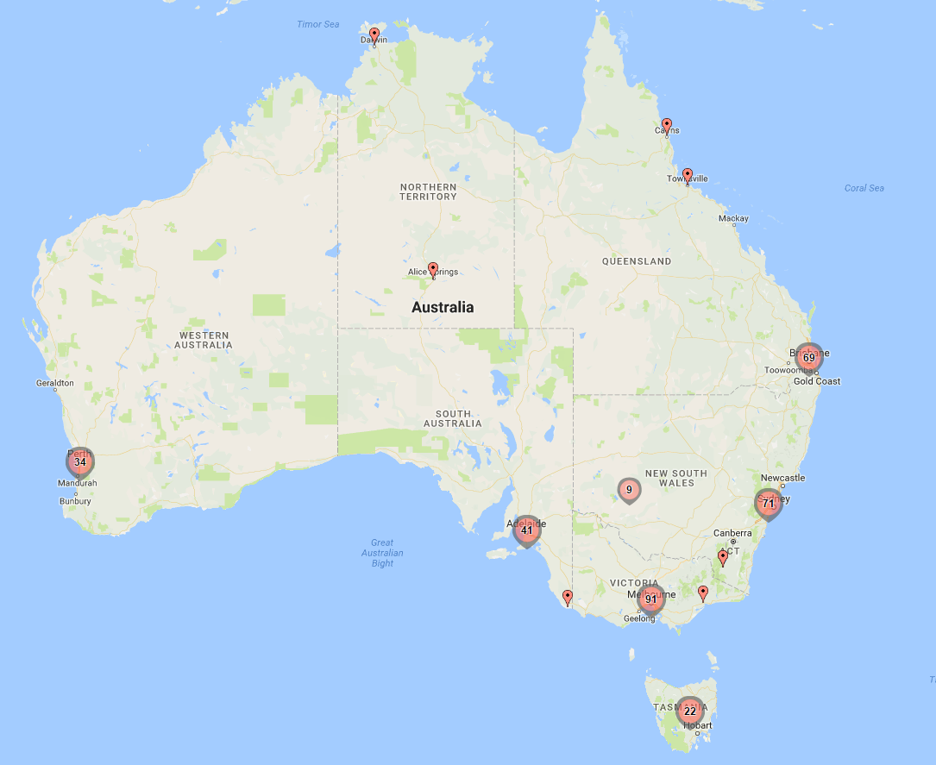
\includegraphics[scale=0.5]{figures/ResponsesMap.png} 
\caption{Locations of Responses}
\label{fig:ResponsesMap}
\end{figure}
Respondents came from all states and territories. While on the map, Figure~\ref{fig:ResponsesMap}, it appears that respondents are clustered around capital cities, this is a function of the scale of the map.



\begin{figure}
\centering
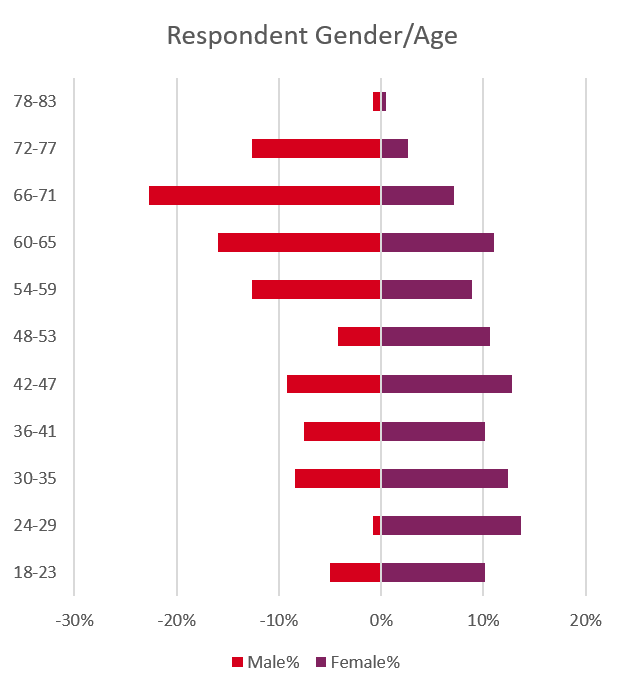
\includegraphics[scale=0.5]{figures/ResponseGender.png} 
\caption{Age and Gender of Respondents}
\label{fig:ResponseGender}
\end{figure}
Figure~\ref{fig:ResponseGender} shows a population pyramid of the age and gender of Respondents. A relatively uniform number of female respondents are seen through almost all age groups, rarely dropping below 10 percent while the age of the male respondents is highly variable and climbs to over double the average of female respondents when the male respondents approach and reach retirement age of 65 before dropping back over 72 years old. This behaviour seems to indicate that women from all age groups were predisposed to take survey this survey but that only men around the age of retirement were. 

\subsection{Technology}
The majority of respondents used the Windows operating system to respond and the majority of those systems were running the latest version of the system, Windows~10. 
\begin{figure}
\centering
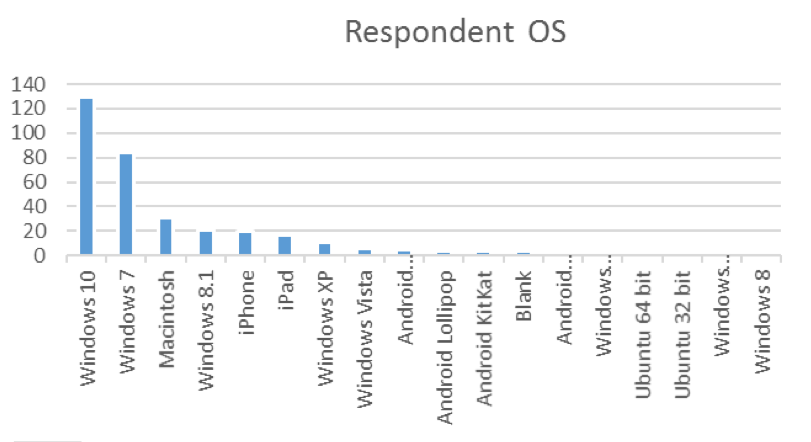
\includegraphics[scale=1]{figures/Survey-OS.png} 
\caption{Operating Systems used by Respondents}
\label{fig:surveyOS}
\end{figure}
Of these respondents, most were using desk-bound computers and majority of these were running the most recent Microsoft Windows operating system, version 10. This information was taken from metadata the browser reported to the survey website. This indicated that very few mobile devices were being used to respond to the survey as there were very few iOS Safari or Android operating systems present in the response data. A very small number of Linux machines were seen in the data but fewer Apple Macintosh systems were found than expected. 


\section{My experiment}
Comparison - qualitative and quantitative difference
\wheelchart{26/mqDarkRed/MQ Dark Red,  28/mqGreyRed/MQ GreyRed, 33.5/mqRed/MQ Red, 12.5/mqPlum!50!mqLightPlum/MQ Plum and Light Plum}\label{fig:GenericExample}

